\documentclass[9pt]{beamer}

\usepackage{amsmath,amssymb,amstext,amsfonts,setspace,dsfont,amsmath,amsthm,array,nomencl,hyperref,pgf,xcolor}

\usepackage{beamerthemesplit}

%\usetheme{Dresden}
\usetheme{Ilmenau}

\setbeamertemplate{navigation symbols}{} %no navigation symbols

\setbeamertemplate{footline}
{%
\leavevmode%
\hbox{%

\begin{beamercolorbox}[wd=.3\paperwidth,ht=2.5ex,dp=1.125ex,left]{author
in head/foot}%
\usebeamerfont{author in head/foot}\hspace{.3cm}\insertshortauthor\hspace{.3cm}
\end{beamercolorbox}%

\begin{beamercolorbox}[wd=.5\paperwidth,ht=2.5ex,dp=1.125ex,center]{title
in head/foot}%
\usebeamerfont{title in head/foot}\hspace{.3cm}\insertshorttitle
\end{beamercolorbox}%

\begin{beamercolorbox}[wd=.2\paperwidth,ht=2.5ex,dp=1.125ex,right]{author
in head/foot}%
\usebeamerfont{author in head/foot}Slide\hspace{.1cm}\insertframenumber\hspace{.1cm}of\hspace{.1cm}\inserttotalframenumber\hspace{.3cm}
\end{beamercolorbox}%
}%
\vskip0pt%
}

\setbeamertemplate{blocks}[rounded][shadow=true]

\title{Linear and Differential Cryptanalysis of DES}
\author{Slava Chernyak and Sourav Sen Gupta}
\institute{University of Washington}
\date{February 2, 2009}

\begin{document}

\begin{frame}
\titlepage
\end{frame}

\section{Introduction}

\begin{frame}
\textit{\huge $\mathcal O$}nce upon a time ... \pause there was a secure standard encryption algorithm called DES (Data Encryption Standard) ...

\vspace{2mm}
\pause
\begin{itemize}[<+->]
\item{1973: NBS publishes a request for a standard encryption algorithm}
\item{1975: DES is published in the Federal Register for comment}
\item{1976: DES is approved as a standard}
\item{1977: DES is published as a FIPS standard FIPS PUB 46}
\item{1992: Biham and Shamir report the {\it differential cryptanalysis}}
\item{1993: DES is reaffirmed for the third time as FIPS 46-2}
\item{1994: The first {\it linear cryptanalysis} of DES is performed by Matsui}
\item{1997: The DESCHALL Project breaks a DES message in public}
\item{1998: The EFF's Deep Crack {\it brute forces} a DES key in 56 hours}
\item{1999: Deep Crack and distributed.net break DES in 22 hours}
\item{1999: FIPS 46-3 reaffirms DES, preferring the use of Triple DES}
\item{2001: The Advanced Encryption Standard (AES) is published in FIPS 197}
\item{2002: The AES standard becomes effective}
\end{itemize}
\end{frame}

\begin{frame}
\tableofcontents
\end{frame}

\begin{frame}
\begin{beamercolorbox}[ht=2.5ex,dp=1.125ex,center,rounded=true,shadow=true]{author in head/foot}
A quick review of DES
\end{beamercolorbox}
\end{frame}

\subsection{Data Encryption Standard}
\begin{frame}
\begin{columns}
\begin{column}{0.6\textwidth}
\begin{block}{DES Function}
DES : (Plaintext ($P$), Key ($K$)) $\mapsto$ Cipher ($C$)
\end{block}

\begin{block}{DES Unit Blocks}
\begin{align*}
\sigma_{i+1} : \: & (0,1)^{64} \rightarrow (0,1)^{64} \\
& (L_i, R_i) \mapsto (L_i \oplus f(R_i,K_{i+1}), R_i) \\
\tau : \: & (0,1)^{64} \rightarrow (0,1)^{64} \\
& (L_{i+1},R_{i+1}) \mapsto (R_{i+1},L_{i+1})
\end{align*}
\end{block}

\begin{itemize}
\item{Input for round $i+1$: $(L_i,R_i)$}
\item{Subkey for round $i+1$: $K_{i+1}$}
\item{Feistel function ($f$)}
\item{16-rounds for $i = 0, 1, ..., 15$}
\end{itemize}

\end{column}

\begin{column}{0.4\textwidth}
\begin{figure}
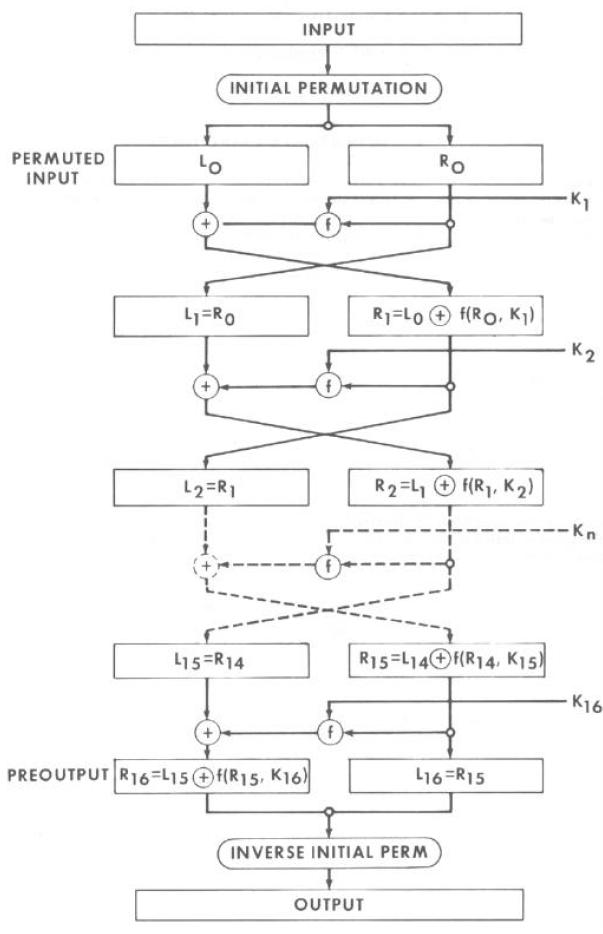
\includegraphics[totalheight=0.8\textheight]{des_algo.jpg}
\caption{DES Algorithm}
\end{figure}
\end{column}
\end{columns}

{\tiny Designers: H Feistel, W Tuchman, D Coppersmith, A Konheim, E Grossman, B Notz, L Smith and B Tuckerman from IBM}
\end{frame}

\begin{frame}
\begin{columns}
\begin{column}{0.45\textwidth}
\begin{block}{Feistel Function}
\begin{align*}
f : \: & (0,1)^{32} \times (0,1)^{48} \rightarrow (0,1)^{32} \\
& (R,K)  \mapsto P (S_{Box}(E(R) \oplus K)) 
\end{align*}
\end{block}

\vspace{0.2in}
\begin{itemize}
\item{Right half of the plaintext ($R$)}
\item{Expansion function \\ $\qquad E : (0,1)^{32} \rightarrow (0,1)^{48}$}
\item{Key for the round ($K$)}
\item{Confusion function (S-Boxes) \\ $\qquad S_i: (0,1)^6 \rightarrow (0,1)^4$}
\item{Diffusion function \\ $\qquad P : (0,1)^{32} \rightarrow (0,1)^{32}$}
\end{itemize}
\end{column}

\begin{column}{0.55\textwidth}
\begin{figure}
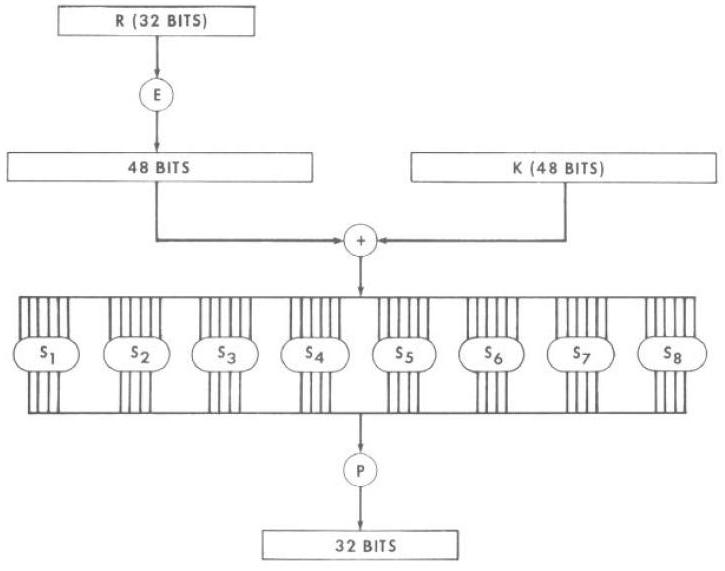
\includegraphics[totalheight=0.6\textheight]{des_feistel.jpg}
\caption{Feistel Round for DES}
\end{figure}
\end{column}
\end{columns}
\end{frame}

\begin{frame}
Mathematically, the different pieces of DES are:

\begin{itemize}
\item{Initial Permutation \\ $\qquad IP : (0,1)^{64} \rightarrow (0,1)^{64}$}
\item{DES Unit Block functions \\ $\qquad \sigma_{i+1} (L_i,R_i)$ for $i = 0,1,...,15$}
\item{Transposition \\ $\qquad \tau : (L_{i+1},R_{i+1}) \mapsto (R_{i+1},L_{i+1})$ for $i = 0,1,...,14$}
\item{Inverse Initial Permutation \\ $\qquad IP^{-1} : (0,1)^{64} \rightarrow (0,1)^{64}$}
\end{itemize}

\pause
\begin{block}{Algebraic Representation of DES}
$\qquad C \:  = \:  DES_K (P) \: = \: IP^{-1} \: \sigma_{16} \:  \tau \: \cdots \:  \tau \:  \sigma_1 \: IP \: (\: P \: )$

$\qquad P \: = \: DES^{-1}_K (C) \: = \: IP^{-1} \: \sigma_{1} \: \tau \: \cdots \: \tau \: \sigma_{16} \: IP \: (\: C\: )$
\end{block}

\pause
\vspace{0.2in}
{\small Note: The inverse DES comes from the fact that $\tau^2 = \sigma_i^2 = 1$}
\end{frame}

\subsection{Linear Cryptanalysis}
\begin{frame}
\begin{beamercolorbox}[ht=2.5ex,dp=1.125ex,center,rounded=true,shadow=true]{author in head/foot}
Basic Idea of Linear Cryptanalysis
\end{beamercolorbox}
\end{frame}

\begin{frame}
Linear Attack on DES idea:

\begin{itemize}[<+->]
\item S-Boxes depend on a relatively small number of bits (6) which allows us to write down linear (or affine) expressions that approximate S-Boxes
\item The effects of one round do not diffuse quickly over following rounds. Thus linear or affine expressions (as above) that hold per-round can be combined across rounds
\end{itemize}
\end{frame}

\begin{frame}
Specifically, if $P_{i}$ are plaintext bits, $C_{i}$ are ciphertext bits, and $K_{i}$ are subkey bits, then we wish to find an expression of the form
\[ P_{i_1} \oplus P_{i_2} \cdots P_{i_j} \oplus C_{i_1} \oplus C_{i_2} \cdots C_{i_k} = K_{i_1} \oplus K_{i_2} \oplus K_{i_m} \]
\pause such that this expression has a high \textit{or} low probability of occurrence.

\vspace{5mm}
\pause Consider: No such obvious expression should exist, otherwise the cipher is trivially weak. If we were to randomly select bits for the above expression, it would hold exactly $1/2$ the time. 

\vspace{5mm}
\pause If we find an expression such as above that displays a high \textit{bias}, that is, it holds much more or less frequently than $1/2$ the time, we can exploit this.
\end{frame}


\subsection{Differential Cryptanalysis}
\begin{frame}
\begin{beamercolorbox}[ht=2.5ex,dp=1.125ex,center,rounded=true,shadow=true]{author in head/foot}
Basic Idea of Differential Cryptanalysis
\end{beamercolorbox}
\end{frame}

\begin{frame}
\begin{definition}[Differential]
Suppose two plaintext inputs to the system be $X$ and $X'$ with corresponding output ciphertexts $Y$ and $Y'$ respectively. 
Then the pair of input difference ($\Delta X = X \oplus X'$) and the output difference ($\Delta Y = Y \oplus Y'$) is called a {\it differential} for the system.
\end{definition}

\vspace{0.2in}
\pause Vulnerability of DES:

\begin{itemize}[<+->]
\item{S-Boxes show a strong tendency to produce certain differential pairs with high probability, rather than being random}
\item{The differences do not get diffused fast enough through the permutations}
\item{Differentials are not affected by the round keys as they get XOR-ed out}
\end{itemize}
\end{frame}

\begin{frame}
In an $k$-round DES, we can trace the path of a certain input difference to get an output difference with a high probability. \pause This tracing path is known as a {\it differential characteristic}.

\[ \Delta P \rightarrow \Delta C^{(1)} \rightarrow \Delta C^{(2)} \rightarrow \cdots \rightarrow \Delta C^{(k-1)} \rightarrow \Delta C \]

\pause In an ideal situation, one will expect the probability
\[ P \left(\Delta C | \Delta P \right) = \frac{1}{2^n} \]
for an $n$-bit cipher system. \pause Differential attacks seek to exploit a scenario where
\[ P \left(\Delta C | \Delta P \right) = p_D \gg \frac{1}{2^n} \]

\pause Note: This is essentially a chosen-plaintext attack as we want the specific input difference to occur for every pair.
\end{frame}

\section{Mathematical Framework}
\begin{frame}
\begin{beamercolorbox}[ht=2.5ex,dp=1.125ex,center,rounded=true,shadow=true]{author in head/foot}
Dive into the Mathematics
\end{beamercolorbox}
\end{frame}

\subsection{Substitution-Permutation Network}

\begin{frame}
\begin{columns}
\begin{column}{0.6\textwidth}
\begin{figure}
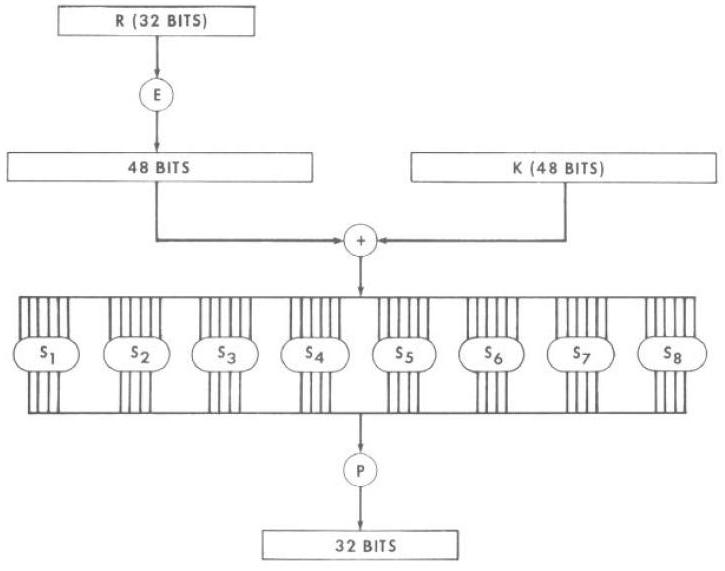
\includegraphics[totalheight=0.5\textheight]{des_feistel.jpg}
\end{figure}
\pause Let us simplify DES by
\begin{itemize}[<+->]
\item{Reducing the code length from $64$ to $16$}
\item{Removing expansion function $E(R)$}
\item{Taking identical S-Boxes of size $4$ bits}
\item{Repeating over less rounds}
\end{itemize}
\end{column}

\begin{column}{0.4\textwidth}
\pause
\begin{figure}
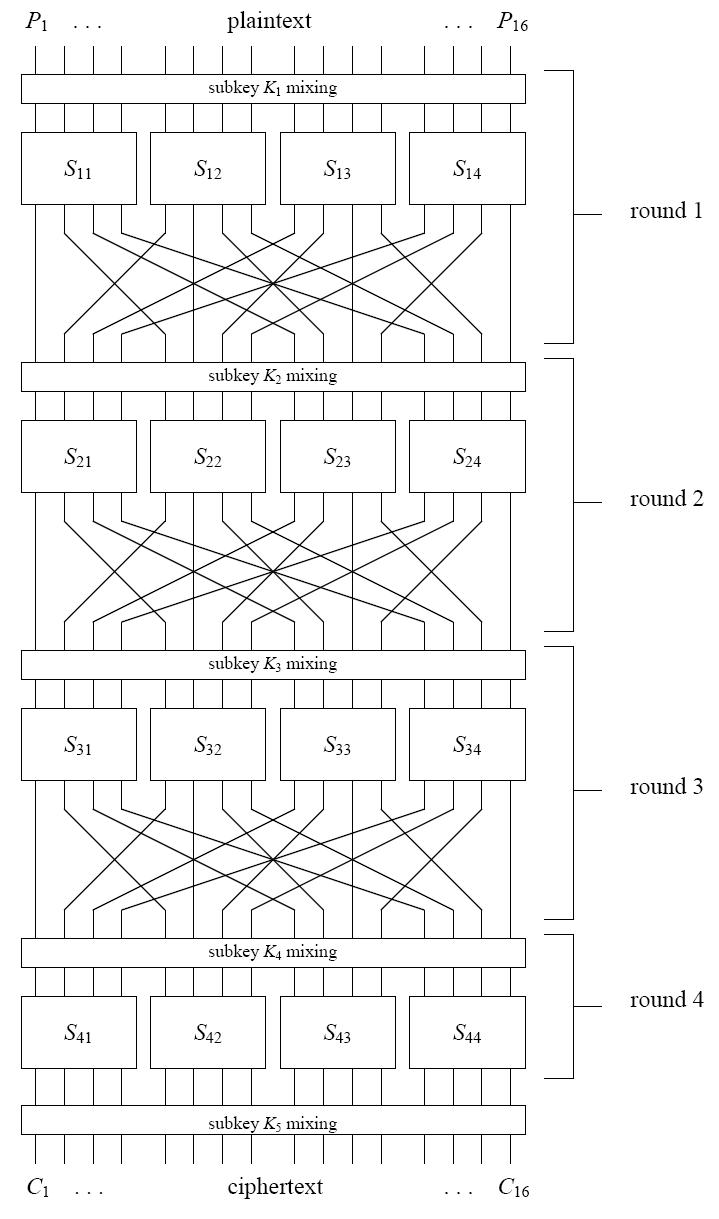
\includegraphics[totalheight=0.8\textheight]{spn.jpg}
\end{figure}
\end{column}
\end{columns}

\begin{center}
\pause {\tiny Disclaimer: This simplification does not affect the discussion of the techniques of Linear/Differential Cryptanalysis.}
\end{center}
\end{frame}

\begin{frame}
\begin{beamercolorbox}[ht=2.5ex,dp=1.125ex,center,rounded=true,shadow=true]{author in head/foot}
Simple Substitution-Permutation Network
\end{beamercolorbox}
\end{frame}

\begin{frame}
We construct a simple Substitution-Permutation Network Cipher (SPN) which has structural similarity to DES.

\begin{itemize}[<+->]
\item SPN is a 16-bit block cipher (16-bit plaintext to 16-bit ciphertext) with 16-bit round keys
\item Each round consists of a substitution and a permutation (much like in DES)
\item The substitution is the result of splitting the 16-bit input block to a round in to 4$\times$4-bit sub-blocks. Each 4-bit sub-block is then mapped across a 4-bit to 4-bit S-Box. We use the same S-Box throughout
\item The permutation is applied to all 16-bits of the round following the substitution
\item Finally, key-mixing is achieved by XOR-ing the round key with every input block to a round as well as at the end of the last round (so that we can't simply ignore the last round)
\item The SPN cipher we will look at will consist of 4 rounds
\end{itemize}
\end{frame}

\begin{frame}
SPN S-Box and Permutation

\vspace{5mm}
SPN uses a single 4-bit S-Box that has the following structure:
\begin{figure}
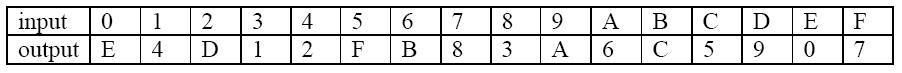
\includegraphics[width=0.9\textwidth]{spn_sbox.jpg}
\end{figure}

\vspace{5mm}
And the following 16-bit permutation:
\begin{figure}
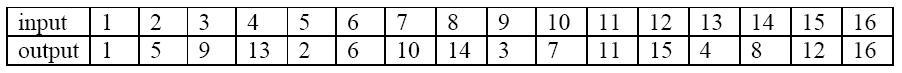
\includegraphics[width=0.9\textwidth]{spn_perm.jpg}
\end{figure}

\vspace{5mm}
\pause The S-Box provides the {\it confusion} function and the permutation applies the {\it confusion} operation in SPN, thus making it cryptographically similar to DES.
\vspace{5mm}

\end{frame}

\subsection{Linear Attack on SPN}
\begin{frame}
\begin{beamercolorbox}[ht=2.5ex,dp=1.125ex,center,rounded=true,shadow=true]{author in head/foot}
Mathematics of Linear Cryptanalysis
\end{beamercolorbox}
\end{frame}

\begin{frame}
Basic Definitions for the Linear attack

\vspace{5 mm}
\pause Linear cryptanalysis tries to take advantage of high probability occurrences of linear expressions involving plaintext bits, ciphertext bits and subkey bits. It is a {\it known plaintext attack}.

\vspace{5 mm}
\pause Define 
\begin{itemize}[<+->]
\item{$P_i$ where $i = 1, 2, \dots 16$ as the $i$-th plaintext bit}
\item{$C_i$ where $i = 1, 2, \dots 16$ as the $i$-th ciphertext bit}
\item{$U_{j,i}$ where $j = 1, 2, 3, 4$ and $i = 1, 2, \dots 16$ be the $i$-th input bit to the $j$-th round of SPN}
\item{$V_{j,i}$ where $j = 1, 2, 3, 4$ and $i = 1, 2, \dots 16$ be the $i$-th output bit of the $j$-th round of SPN}
\end{itemize}
\end{frame}

\begin{frame}
Linear and Affine approximation of S-Box

\vspace{5mm}
\begin{itemize}[<+->]
\item Question: How do we come up with the desired expression for the entire cipher? 
\item Hint: We start by looking at the only non-linear component, the S-Box.
\end{itemize}

\vspace{5mm}
\pause To find the linear/affine approximation of the S-Box we simply consider every possible expression of the input bits $X_i$ and output bits $Y_j$. \pause Thus the expression has the form
\[ \bigoplus_{i \in U} X_i = \bigoplus_{j \in V} Y_j \]
where $U$ and $V$ range over all possible subsets of $\{1, 2, 3 ,4\}$. \pause We then compare how often this expression coincides with the S-Box.

\vspace{5mm}
\pause Note that there are 16 possibilities for $U$ and $V$, hence 256 total possible expressions (for a 4-bit S-box).
\end{frame}

\begin{frame}
S-Box Approximation Example

\vspace{5mm}
\begin{columns}
\begin{column}{0.3\textwidth}
\begin{figure}
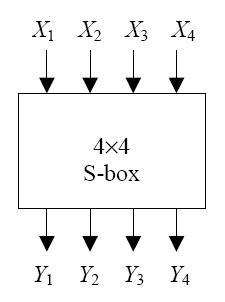
\includegraphics[width=0.7\textwidth]{spn_sbox_unkeyed.jpg}
\end{figure}
\end{column}

\begin{column}{0.7\textwidth}
We can take the following expression as an example:
\[ X_2 \oplus X_3 = Y_1 \oplus Y_3 \oplus Y_4 \]
\pause Applying all possible values for the input $X$ bits it turns out that the expression holds in 12 out of the 16 cases. \pause Hence, this expression has a bias of $12/16 - 1/2 = 1/4$.
\end{column}
\end{columns}

\vspace{5mm}
\pause Similarly the following expression
\[ X_3 \oplus X_4 = Y_1 \oplus Y_4 \]
Has a bias of $-3/8$, which is higher in magnitude than the previous one. \pause It is the magnitude of the bias that is important.
\end{frame}

\begin{frame}
The number of agreements (minus 8) between the S-Box and every possible expression is summarized in the table below. Thus to get the bias, one must only divide by 16.

\vspace{5mm}
\begin{figure}
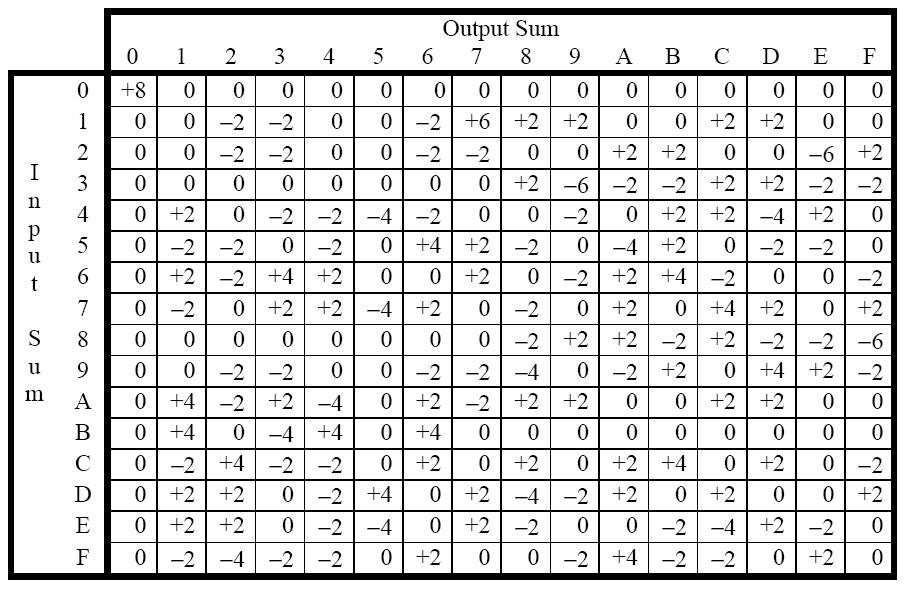
\includegraphics[height=0.7\textheight]{spn_linear_approx.jpg}
\end{figure}
\end{frame}


\begin{frame}
\begin{columns}
\begin{column}{0.4\textwidth}
What this means for 1 Round:

\vspace{5mm}
Note, from the previous table, that the expression \[ X_1 \oplus X_3 \oplus X_4 = Y_2 \] has a bias of $+1/4$.

\vspace{5mm}
\onslide<2->{Note also that $U_1 = P \oplus K_1$.}
\end{column}
\begin{column}{0.6\textwidth}
\begin{figure}
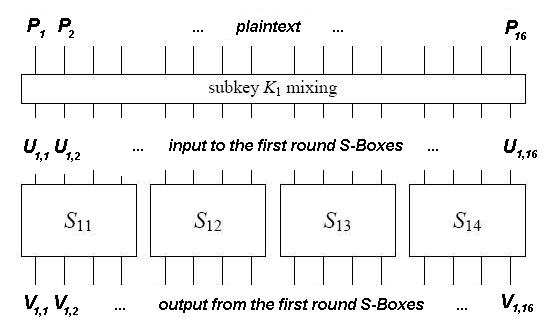
\includegraphics[height=0.45\textheight]{spn_single_round.jpg}
\end{figure}
\end{column}
\end{columns}

\vspace{5mm} 
\onslide<3->{We can now write down the following linear approximation across the 1st round of SPN:
\begin{eqnarray*}
V_{1,6} & = & U_{1,5} \oplus U_{1,7} \oplus U_{1,8} \quad \mbox{  $\leftarrow$ S-Box $S_{12}$ approximation above}\\
		  & = & (P_5\oplus K_{1,5}) \oplus (P_7\oplus K_{1,7}) \oplus (P_8\oplus K_{1,8})
\end{eqnarray*}

\pause This expression holds with probability of $3/4$ (bias of $+1/4$)}
\end{frame}

\begin{frame}
We can get expressions that hold with some non-$1/2$ probability for every round. But we must somehow combine them to write an expression relating the plaintext and ciphertext bits. \pause We use the Piling Up Principle for this purpose.

\vspace{5mm}
\pause Note:

$\qquad X_1 \oplus X_2 = 0$ is a linear expression equivalent to $X_1 = X_2$\\
$\qquad X_1 \oplus X_2 = 1$ is an affine expression equivalent to $X_1 \neq X_2$

\vspace{5mm}
\pause Assume the following probability distribution
\[ Pr(X_1 = i)  = \left\{ \begin{array}{ll}
         p_1 & \mbox{$i = 0$};\\
         (1 - p_1) & \mbox{$i = 1$}.\end{array} \right. \] 
\[ Pr(X_2 = i)  = \left\{ \begin{array}{ll}
         p_2 & \mbox{$i = 0$};\\
         (1 - p_2) & \mbox{$i = 1$}.\end{array} \right. \] 
\end{frame}

\begin{frame}
Piling Up Principle (continued):

\vspace{5mm}
Assuming that $X_1$ and $X_2$ are independent, we get
\[ Pr(X_1 = i, X_2 = j)  = \left\{ \begin{array}{ll}
         p_1 p_2 & \mbox{$i = 0, j = 0$};\\
         (1 - p_1) p_2 & \mbox{$i = 1, j = 0$} \\
			p_1 (1 - p_2) & \mbox{$i = 0, j = 1$} \\
			(1 - p_1)(1 - p_2) & \mbox{$i = 1, j = 1$}.\end{array} \right. \] 
\pause Now, note that $X_1 \oplus X_2 = 0 \Rightarrow X_1 = 1, X_2 =1$ OR $X_1 = 0, X_2 = 0$. \pause Hence,
\begin{eqnarray*}
 Pr(X_1 \oplus X_2 = 0) & = & Pr(X_1=0,X_2=0) + Pr(X_1=1,X_2=1) \\
								& = & p_1p_2 + (1 - p_1)(1-p_2)
\end{eqnarray*}
\pause If we write $p_k = 1/2 + \epsilon_k$ we have
\[ Pr(X_1 \oplus X_2 = 0) = 1/2 + 2\epsilon_1 \epsilon_2 \]
\pause Hence the bias of $X_1 \oplus X_2 = 0$ is 
\[ 2 \epsilon_1 \epsilon_2 \]
That is, twice the product of the bias of the original expressions.
\end{frame}

\begin{frame}
Piling Up Principle (continued) - The Piling Up Lemma:\\
\vspace{5mm}
We extend the idea on the previous slide to the general case \pause : For $n$ independent random binary variables, $X_1, X_2, \dots, X_n$, 
\[ Pr(X_1 \oplus X_2 \cdots \oplus X_n = 0) = 1/2 + 2^{n-1} \prod_{i=1}^n \epsilon_i \]
\pause In terms of bias,
\[ \epsilon_{1,2,\dots,n} = 2^{n-1} \prod_{i = 1}^n \epsilon_i \]
Where $\epsilon_{1,2,\dots,n}$ is the total bias of $X_1 \oplus X_2 \cdots \oplus X_n = 0$. \\
\vspace{5mm}
\pause Note that if some $\epsilon_k = 0$ (that is, some $X_k$ has no bias) then total bias will be $0$. More about the probabilistic analysis later.
\end{frame}

\begin{frame}

\begin{columns}
\begin{column}{0.6\textwidth}
Now, come back to per-round approximations. We can write down 4 approximations ($S_{ij}$ represents the $j$-th S-Box in the $i$-th round):
\begin{align*}
& S_{12}: X_1 \oplus X_3 \oplus X_4 = Y_2 \\
& S_{22}: X_2 = Y_2 \oplus Y_4 \\
& S_{32}: X_2 = Y_2 \oplus Y_4 \\
& S_{34}: X_2 = Y_2 \oplus Y_4 \\
\end{align*}
\onslide<2->{Each of these has a probability bias magnitude of $1/4$. We can use the Piling Up Principle to combine them into a single expression relating plaintext bits to ciphertext bits.}
\end{column}

\begin{column}{0.4\textwidth}
\begin{figure}
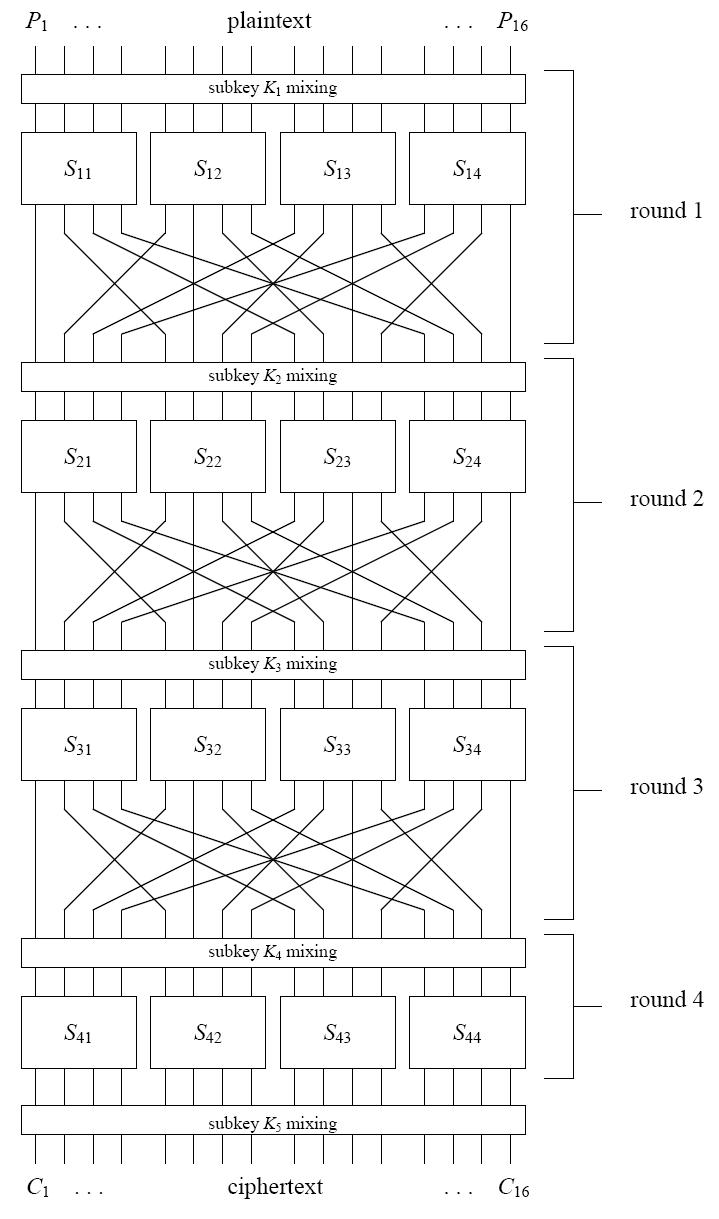
\includegraphics[totalheight=0.8\textheight]{spn.jpg}
\end{figure}
\end{column}
\end{columns}

\end{frame}

\begin{frame}
\begin{columns}
\begin{column}{0.6\textwidth}
Consider the first 2 rounds:
\begin{align*}
& X_1 \oplus X_3 \oplus X_4 = Y_2 \\ 
\Rightarrow &(P_5\oplus K_{1,5}) \oplus (P_7\oplus K_{1,7}) \oplus (P_8\oplus K_{1,8}) =  V_{1,6}
\end{align*}
\[ X_2 = Y_2 \oplus Y_4 \: \Rightarrow \: (V_{1,6} \oplus K_{2,6}) =  V_{2,6} \oplus V_{2,8}\]

\vspace{2mm}
\onslide<2->{Each of these has a bias of magnitude $1/4$ and we can combine to obtain:
\[ V_{2,6} \oplus V_{2,8} \oplus P_5 \oplus P_7 \oplus P_8 \oplus K_{1,5} \oplus K_{1,7} \oplus K_{1,8} \oplus K_{2,6} = 0 \]}

\vspace{2mm}
\onslide<3->{By the Piling Up Principle this holds with bias
\[ 2 \times 1/4 \times 1/4 = 1/8 \]}
\end{column}

\begin{column}{0.4\textwidth}
\begin{figure}
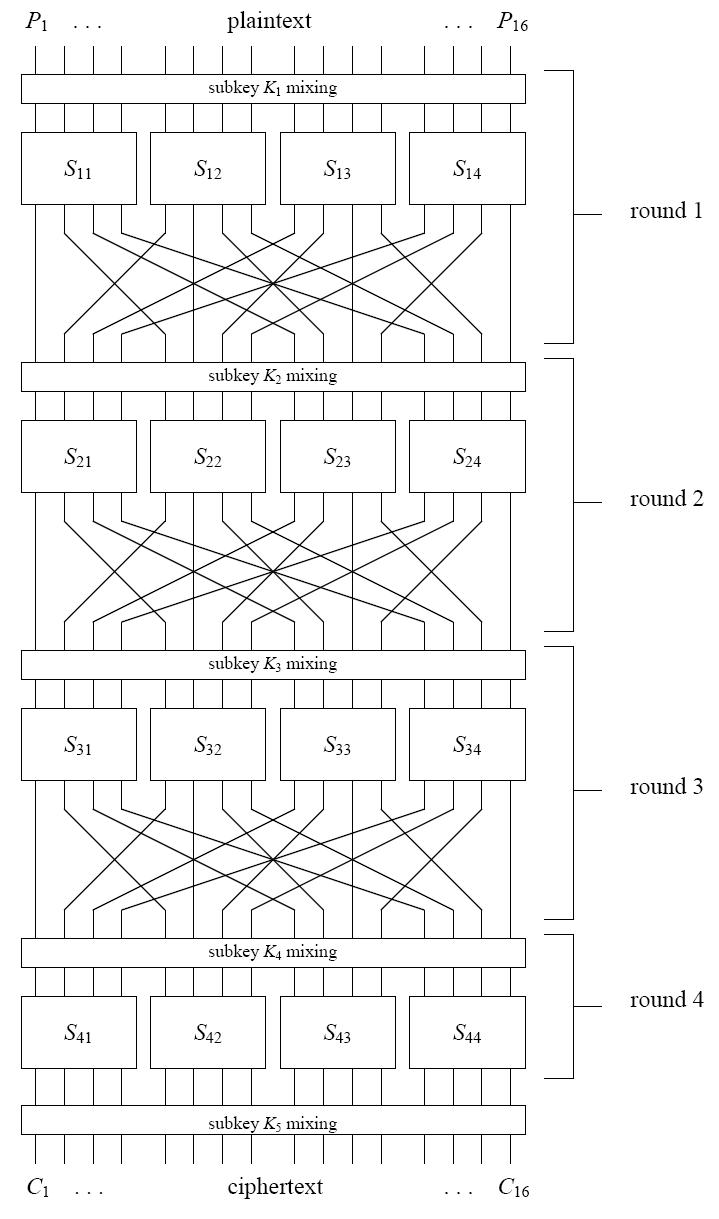
\includegraphics[totalheight=0.8\textheight]{spn.jpg}
\end{figure}
\end{column}
\end{columns}

\vspace{2mm}
\onslide<4->{Note the implicit assumption that S-Boxes are independent. More on this later.}

\end{frame}

\begin{frame}
Using this principle we can write the following equation over 3 rounds of SPN:
\[ U_{4,6} \oplus U_{4,8} \oplus U_{4,14} \oplus U_{4, 16} \oplus P_5 \oplus P_7 \oplus P_8 = \Sigma K \]
\pause Where $\Sigma K$ is the sum over some key bits. Note that Since the key is fixed, $\Sigma K = 0$ or $1$ and thus we can ignore it since we only care about the bias.\\
\vspace{5mm}
\pause The magnitude of the bias of the above expression, by the Piling Up Principle, is $1/32$. \\
\vspace{5mm}
\pause Next we show how we can extract key bits using this information.
\end{frame}

\begin{frame}
Attack Idea:\\
\vspace{3mm}
We have an expression that links plaintext bits to input bits to the 4th round of SPN that holds with high bias ($1/32$). 
\[ U_{4,6} \oplus U_{4,8} \oplus U_{4,14} \oplus U_{4, 16} \oplus P_5 \oplus P_7 \oplus P_8 = \Sigma K \]
\pause We can partially undo the last round by guessing the last key. \\
\vspace{3mm}
\pause
If we guess correctly, the equation will hold with high bias. If we guess wrong, the equation will probably hold with probability close to 1/2, that is, a bias close to 0.\\
\vspace{3mm}
\pause
BUT To do this, we don't need to guess the entire key for the last round! \pause Our expression only involves 4 fourth round input ($U_4$) bits, output from 2 S-Boxes of the third round. Thus we only need to guess $2^8 = 256$ values.\\
\vspace{3mm}
\pause
For each value of the guessed \textit{target partial subkey} we can undo the last round and determine the bias of the equation. Highest bias indicates likely correct guess.
\end{frame}

\begin{frame}
\begin{columns}
\begin{column}{0.45\textwidth}
\begin{block}{SPN Linear Approximation}
\begin{align*}
 U_{4,6} & \oplus U_{4,8} \oplus U_{4,14} \oplus U_{4, 16} \\
         & \oplus P_5 \oplus P_7 \oplus P_8 = 0 
\end{align*}
\end{block}
\end{column}
\begin{column}{0.55\textwidth}
\begin{figure}
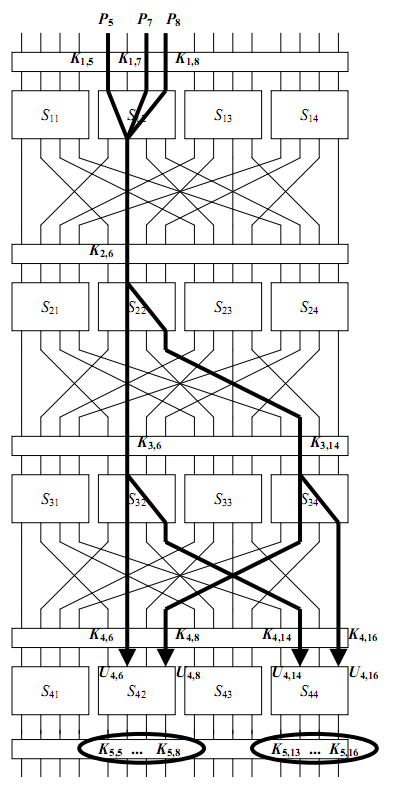
\includegraphics[totalheight=0.85\textheight]{SPN_linear.PNG}
\caption{Linear Attack on SPN}
\end{figure}
\end{column}
\end{columns}
\end{frame}

\begin{frame}
Probabilistic justification for number of pairs:\\
\vspace{5mm}
\pause In general, the number of plaintext-ciphertext pairs needed is related inversely-quadratically to the bias. That is
\[ N_{pairs} \approx 1 / \epsilon^2 \]
\pause For the SPN cipher approximation with bias $1/32$ we need about $1000$ pairs to perform the attack with near full probability of success.
\end{frame}

\begin{frame}
Actual attack on SPN ... Demo ...
\end{frame}

\subsection{Differential Attack on SPN}
\begin{frame}
\begin{beamercolorbox}[ht=2.5ex,dp=1.125ex,center,rounded=true,shadow=true]{author in head/foot}
Mathematics of Differential Cryptanalysis
\end{beamercolorbox}
\end{frame}

\begin{frame}
Differential: $(\Delta P, \Delta C) = (P \oplus P', C \oplus C')$

\vspace{5mm}
\pause Differential Cryptanalysis tries to exploit the high probability of certain occurrences of differential characteristics $(\Delta P \rightarrow \Delta C)$ in the cipher. 

\vspace{2mm}
\pause Note: This is a chosen plaintext attack.

\vspace{5mm}
\pause We have to analyze the cipher in pieces. \pause The basic idea is
\begin{itemize}[<+->]
\item{Analyze the difference pattern and their probabilities of the S-Box}
\item{Combine the S-Boxes over the rounds to build the differential characteristic of the cipher}
\item{Choose the characteristic with maximum probability and use that to retrieve subkey bits of the cipher}
\end{itemize}
\end{frame}

\begin{frame}
Analyzing the S-Box

\vspace{2mm}
Let us consider the S-Box of the SPN cipher as we constructed it:
\begin{columns}
\begin{column}{0.5\textwidth}
\begin{itemize}
\item{$4 \times 4$ S-Box}
\item{Input: $X = [X_1 \: X_2 \: X_3 \: X_4]$}
\item{Output: $Y = [Y_1 \: Y_2 \: Y_3 \: Y_4]$}
\item{Difference pair: $(\Delta X, \Delta Y)$}
\end{itemize}
\end{column}
\begin{column}{0.5\textwidth}
\begin{figure}
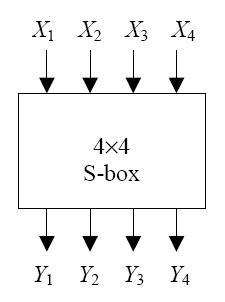
\includegraphics[totalheight=0.3\textheight]{spn_sbox_unkeyed.jpg}
\end{figure}\end{column}
\end{columns}

\vspace{2mm}
\pause Algorithm
\begin{enumerate}[<+->]
\item{Fix a certain input difference $\Delta X = 0100$, say}
\item{Iterate through the first input $X = \{0000, ... ,1111 \}$}
\item{This fixes the second input $X' = X \oplus \Delta X = \{0100, ... ,1011\}$ (ordering does not matter)}
\item{Obtain corresponding output difference $\Delta Y = Y \oplus Y'$}
\item{Iterate through steps 2 to 4 for $\Delta X = \{0000, ... ,1111 \}$} 
\end{enumerate}
\end{frame}

\begin{frame}
Sample Difference Pairs for the S-Box

\begin{figure}
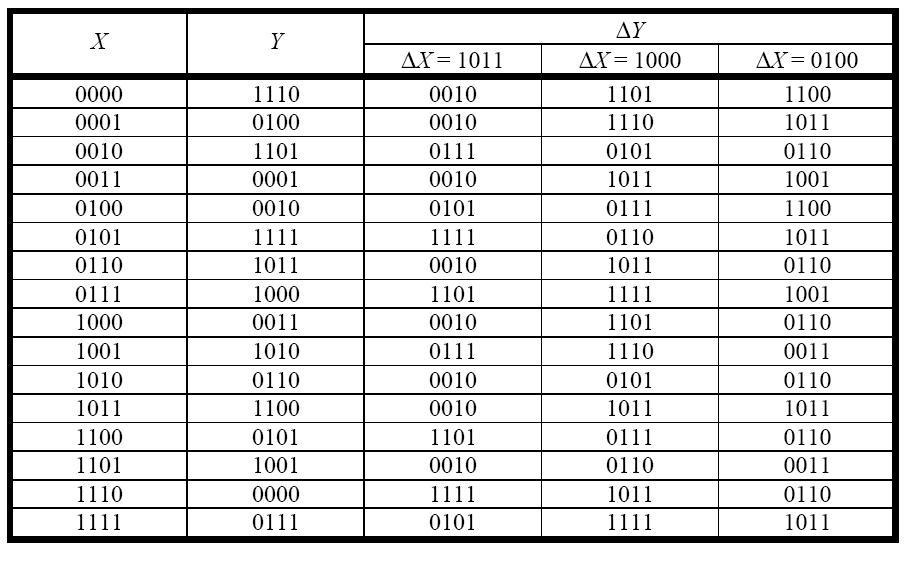
\includegraphics[totalheight=0.6\textheight]{spn_sbox_diffpairs.jpg}
\end{figure}

\pause Note that, for $\Delta X = 1011$, $\Delta Y = 0010$ occurs $8$ times, out of the possible $16$ times. So, the pair $(1011,0010)$ has a probability of occurrence $8/16 = 1/2$. 

\vspace{2mm}
\pause We can tabulate the complete data for the S-Box to check this probabilities.
\end{frame}

\begin{frame}
Difference Distribution Table

\begin{figure}
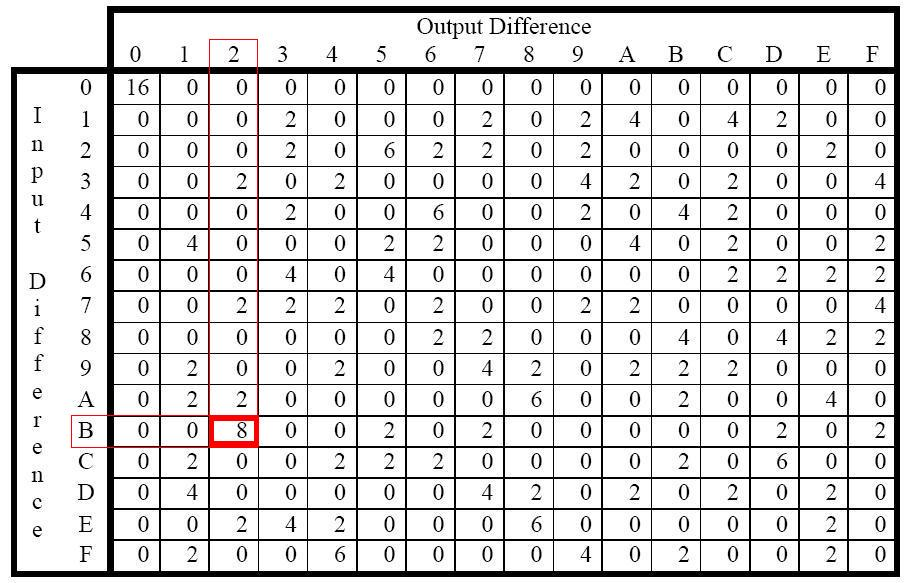
\includegraphics[totalheight=0.6\textheight]{spn_sbox_disttable.jpg}
\end{figure}

\pause Note that
\begin{itemize}[<+->]
\item{In an ideal S-Box, we would like all entries to be $1$}
\item{But this table clearly shows bias towards certain pairs}
\item{Just divide the entries by $2^4 = 16$ to get the probabilities, and exploit the scenario of highest probability of occurrence ($Pr(2|B) = 8/16 = 1/2$ here)}
\end{itemize}
\end{frame}

\begin{frame}
A few properties of the S-Box Distribution Table

\vspace{5mm}
\pause Notice that in the difference table
\begin{itemize}[<+->]
\item{The $(0,0)$ entry is $16$, just because identical inputs ($\Delta X = 0 \Rightarrow X = X'$) should produce identical outputs ($Y = Y' \Rightarrow \Delta Y = 0$)}
\item{All the entries are even, because $\Delta X$ is the same for both the input pairs $(X,X')$ and $(X',X)$, producing same $\Delta Y$}
\item{Sum of all entries in a row is $2^4 = 16$}
\end{itemize}

\vspace{5mm}
\pause As an ideal S-Box expects to give out no information of $\Delta Y$ given $\Delta X$, we wish it could have all entries $1$, i.e,
\[ Pr(\Delta Y | \Delta X) = \frac{1}{16} \quad \forall \: \Delta X  \]
\pause But, from our discussion above, this is infeasible, and we hope to exploit this.
\end{frame}

\begin{frame}
What happens for a Keyed S-Box?

\vspace{5mm}
\pause Let us consider the S-Box of the SPN cipher, with the round keys this time.
\pause
\begin{columns}
\begin{column}{0.5\textwidth}
\begin{itemize}
\item{$4 \times 4$-bit S-Box}
\item{Input: $W = [W_1 \: W_2 \: W_3 \: W_4]$}
\item{Round Key: $K = [K_1 \: K_2 \: K_3 \: K_4]$}
\item{Output: $Y = [Y_1 \: Y_2 \: Y_3 \: Y_4]$}
\item{Difference pair: $(\Delta W, \Delta Y)$}
\end{itemize}
\end{column}
\begin{column}{0.5\textwidth}
\begin{figure}
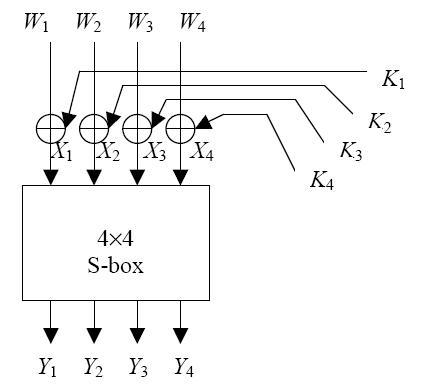
\includegraphics[totalheight=0.3\textheight]{spn_sbox_keyed.jpg}
\end{figure}
\end{column}
\end{columns}

\vspace{5mm}
\pause Note that for each pair of inputs $(W,W')$, the actual inputs to the S-Box are $(X,X') = (W \oplus K, W' \oplus K)$. Hence, the input difference for the keyed S-Box is 
\[ \Delta W = W \oplus W' = (X \oplus K) \oplus (X' \oplus K) = X \oplus X' = \Delta X \]
\pause and hence $\Delta W \rightarrow \Delta Y$ corresponds identically to $\Delta X \rightarrow \Delta Y$.

\vspace{2mm}
\pause Thus, the keyed S-Box has the same difference distribution table.
\end{frame}

\begin{frame}

\begin{columns}
\begin{column}{0.4\textwidth}
\begin{figure}
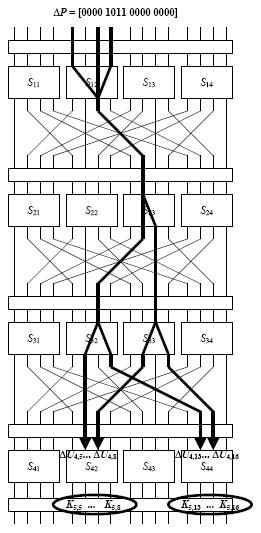
\includegraphics[totalheight=0.8\textheight]{spn_diff_char.jpg}
\end{figure}
\end{column}

\begin{column}{0.6\textwidth}
Constructing a Differential Characteristic

\vspace{5mm}
\pause The diagram beside illustrates the tracing of the non-zero bits of the input difference through the SPN structure.

\vspace{2mm}
Input Difference: $\Delta P = 0B00$

\vspace{2mm}
\pause Propagating Difference Pairs
\begin{itemize}[<+->]
\item{$S_{12}$: $1011 \rightarrow 0010$ [$Pr = \frac{8}{16}$]}
\item{$S_{23}$: $0100 \rightarrow 0110$ [$Pr = \frac{6}{16}$]}
\item{$S_{32}$: $0010 \rightarrow 0101$ [$Pr = \frac{6}{16}$]}
\item{$S_{33}$: $0010 \rightarrow 0101$ [$Pr = \frac{6}{16}$]}
\item{$S_{ij}$: $0000 \rightarrow 0000$ [$Pr = \frac{16}{16}$]}
\end{itemize}

\vspace{2mm}
\pause Differential Characteristic
\[ 0B00 \rightarrow 0040 \rightarrow 0220 \rightarrow 0606 \]
\end{column}
\end{columns}
\end{frame}

\begin{frame}
Piling up Probabilities

\vspace{2mm}
\pause Notation
\begin{itemize}
\item{$\Delta U_i$: Input difference to $i$-th round}
\item{$\Delta V_i$: Output difference from $i$-th round}
\item{$K_i$: Round Key for $i$-th round}
\item{$X_{i,j}$: $j$-th bit of $X_i$}
\end{itemize}

\vspace{2mm}
\pause Here, we have the following in the differential characteristic
\begin{itemize}[<+->]
\item{Round 1: $\Delta P = \Delta U_1 = 0B00 \rightarrow 0040 = \Delta V_1$  [$Pr = 8/16$]}
\item{Round 2: $\Delta V_1 = \Delta U_2 = 0040 \rightarrow 0220 = \Delta V_2$  [$Pr = 6/16$]}
\item{Round 3: $\Delta V_2 = \Delta U_3 = 0220 \rightarrow 0606 = \Delta V_3$  [$Pr = \left(6/16\right)^2$]}
\item{Round 4: $\Delta V_3 = \Delta U_4 = 0606$}
\end{itemize}

\vspace{2mm}
\pause Hence, assuming the S-Boxes to be independent over the rounds, we obtain
\[ \Delta P = 0B00 \rightarrow 0606 = \Delta U_4 \]
with probability $Pr(\Delta U_4 | \Delta P) = 8/16 \times 6/16 \times \left(6/16\right)^2 = 27/1024$.

\vspace{2mm}
\pause Note: The probability of this characteristic $Pr = 27/1024 \gg 1/2^{16}$

\end{frame}

\begin{frame}
Attack Idea
\begin{itemize}[<+->]
\item{We have a differential characteristic that links plaintext difference $\Delta P$ to input difference $\Delta U_4$ of the 4th round output of SPN and holds with high probability ($27/1024$)}
\item{We can partially undo the last round by guessing the last key $K_5$}
\item{If we guess correctly, the differential characteristic will hold with high probability, close to $27/1024$. If we guess wrong, it will hold with low probability}
\item{But in this case, we don't need to guess the entire key $K_5$ for the last round!}
\item{The differential output only involves 2 S-Boxes, $S_{42}$ and $S_{44}$. Thus we only need to guess $2^8 = 256$ values}
\item{For each value of the guessed \textit{target partial subkey} we can undo the last round and determine the probability of the differential characteristic}
\item{Highest probability indicates likely correct guess}
\end{itemize}

\end{frame}

\begin{frame}
\begin{columns}
\begin{column}{0.4\textwidth}
\begin{figure}
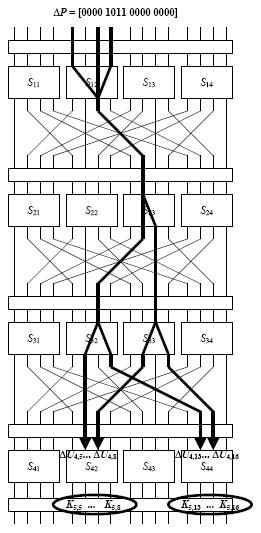
\includegraphics[totalheight=0.8\textheight]{spn_diff_char.jpg}
\end{figure}
\end{column}

\begin{column}{0.6\textwidth}
Differential Characteristic flow

\vspace{5mm}
\pause Input Difference: $\Delta P = 0B00$ 

\vspace{2mm}
\pause Characteristic
\[ \Delta P = 0B00 \rightarrow 0606 = \Delta U_4 \]

\vspace{2mm}
Probability $Pr(\Delta U_4 = 0606 | \Delta P = 0B00) = 27/1024$

\vspace{5mm}
\pause Partial Subkey guess only for
\[ [K_{5,5} ... K_{5,8}, K_{5,13} ... K_{5,16}] \]
\end{column}
\end{columns}

\end{frame}

\begin{frame}
Actual attack on SPN ... Demo ...
\end{frame}

\begin{frame}
\begin{beamercolorbox}[ht=2.5ex,dp=1.125ex,center,rounded=true,shadow=true]{author in head/foot}
It's time for a Break!
\end{beamercolorbox}
\end{frame}


\section{Attacks on DES}
\begin{frame}
\begin{beamercolorbox}[ht=2.5ex,dp=1.125ex,center,rounded=true,shadow=true]{author in head/foot}
Do these work for DES?
\end{beamercolorbox}
\end{frame}

\subsection{Linear Attack: 4-round DES}
\begin{frame}
The plan for the DES Attacks:
\begin{itemize}
\item{Structurally and cryptographically, DES is similar to SPN.}
\item{We will adapt the linear attack on SPN to a linear attack on a 4-round DES algorithm and mount this attack.}
\item{We will also show how to extend this attack to a full 16-round DES algorithm and show it is faster than an exhaustive search.}
\end{itemize}
\end{frame}

\begin{frame}
The first step, as before, is to come up with a linear approximation for the S-Boxes used by DES.\\
\vspace{5mm}
Note that the S-Boxes here are 6-bit to 4-bit maps. We can use the same technique as before. For a given S-Box $a \in \{1, 2, \dots 8\}$, $1 \leq \alpha \leq 63$, $1 \leq \beta \leq 15$, we define $NS_{a}(\alpha, \beta)$ as the number of times (out of 64) for S-Box $a$ that for all the input patterns masked by $\alpha$ the output pattern masked by $\beta$ agrees with the value of S-Box $a$.
\[ NS_{a}(\alpha, \beta) = | \{ X | 0 \leq X < 64, ( \bigoplus_{i=0}^5 X[i]\cdot\alpha[i]) = (\bigoplus_{j=0}^3 S_a(X)[j] \cdot \beta[j])\} | \]
This looks more complicated, but is in fact the same expression as for SPN, except it takes into account all possible S-Boxes.
\end{frame}

\begin{frame}
Using $NS$ to find a linear approximation for the S-Boxes.\\
\vspace{5mm}
With 6-bit S-Boxes things are not as easy as with 4-bit S-Boxes.
\begin{figure}
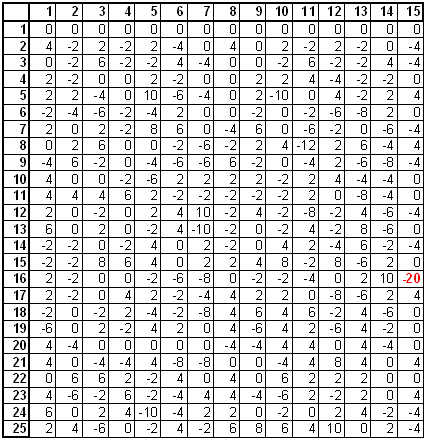
\includegraphics[totalheight=0.5\textheight]{NS_S5.PNG}
\caption{Bias for S-Box 5 }
\end{figure}
It turns out that the highest bias is for S-Box 5 with $\alpha = 16$ and $\beta = 15$
\end{frame}

\begin{frame}
From previous result, the S-Box approximation with highest bias for S-Box 5. Let $X$ be the input bits to the S-Box and let $Y$ be the output bits. Then:
\[ X_{2} = Y_{1} \oplus Y_{2} \oplus Y_{3} \oplus Y_{4} \]
Holds with bias of absolute value $\sim 0.31$\\
\vspace{5mm}
Tracing through the Feistel function to the right input bits $R$, round key bits $K$, and Feistel function output bits $F$ we get
\[ R_{17} \oplus F_{25} \oplus F_{14} \oplus F_{8} \oplus F_{3} = K_{26} \]

\end{frame}

\begin{frame}
Let $P_L$ and $P_R$ be the left and right plaintext bits. Let $C_L$ and $C_R$ be the left and right ciphertext bits. Let $K_i$ be the round key for round $i$ and $U_{4L}$ and $U_{4R}$ the left and right halves of the input to round 4.\\
\vspace{5mm}
Using the S-Box 5 approximation and the Piling Up Principle we can combine the approximations to get
\begin{align*}
 P_L[25] & \oplus P_L[14] \oplus P_L[8] \oplus P_L[3] \oplus \\
         & U_{4L}[25] \oplus U_{4L}[14] \oplus U_{4L}[8] \oplus U_{4L}[3] \oplus \\
			& P_R[17] \oplus U_{4R}[17] = K_1[26] \oplus K_3[26] \\
\end{align*}
The bias magnitude for this expression is
\[ (12/64)^2 + (1 - 12/64)^2 - 1/2 \approx 0.30 \]
This is the best expression for the 3-round DES.
\end{frame}

\begin{frame}
We perform the attack on the 4-round DES similarly to how we performed the attack on 4-round SPN, by ``undoing'' the last round.\\
\vspace{5mm}
\pause
Note that in the last round, $U_{4L}$ bits are not changed, only $U_{4R}$ bits are affected. Note also that there is only one $U_R$ bit the 3-round equation.
\begin{align*} 
P_L[25] \oplus P_L[14] \oplus P_L[8] \oplus & P_L[3] \oplus U_{4L}[25] \oplus U_{4L}[14] \oplus U_{4L}[8] \\ & \oplus U_{4L}[3] \oplus P_R[17] \oplus U_{4R}[17] = K_1[26] \oplus K_3[26]
\end{align*}
\vspace{5mm}
\pause
This bit, $U_{4R}[17]$ is affected by the result of S-Box 1 in round 4. If we guess correctly for the 6 partial subkey bits $K_{4,1}$ to $K_{4,6}$, the 3-round equation will hold with high bias, otherwise it will likely hold with close to 0 bias.\\
\vspace{5mm}
\pause
Thus, this attack will give us $6$ of the $56$ key bits. What this means in terms of time saved over exhaustive search is this: If it takes a year to find a key through exhaustive search of $2^{56}$ bits, after this attack it will only take $5$ days to exhaustively search the remaining $2^{50}$ bits.
\end{frame}

\begin{frame}
How many pairs do we need? (Probabilistic justification)

\vspace{3mm}
Matsui Lemma 5: Let $N$ be the number of given random plaintexts and $\epsilon$, the bias, be sufficiently small. Let $q^{(i)}$ be the probability that the following equation holds for a subkey candidate $K_n^{(i)}$ and a random variable X:
\[ F_n(X,K_n)[l_1, l_2,\dots,l_d] = F_n(X, K_n^{(i)})[l_1, l_2, \dots, l_d].\]
Then if $q^{(i)}$'s are independent, the success rate of the attack is
\[ \int_{x=-2\sqrt{N}\epsilon}^\infty \left( \prod_{K_n^{(i)} \neq K_n} \int_{-x-4\sqrt{N}\epsilon q^{(i)}}^{x+4\sqrt{N}\epsilon (1 - q^{(i)})} \frac{1}{\sqrt{2\pi}} e^{-y^2/2} dy \right) \frac{1}{\sqrt{2\pi}} e^{-x^2/2} dx \]
Where the product is taken over all subkey candidates except $K_n$.\\
\vspace{3mm}
Let $d = 1$ and $l_1 = 17$ in the above expression - this corresponds to our attack (distribution over guessing for one bit, $CR_{17}$ in the equation). The following table summarizes the success rates:
\begin{center}
\begin{tabular}{|c|r|r|r|r|}
\hline
N & 2$\epsilon^{-2}$ & $4\epsilon^{-2}$ & $8\epsilon^{-2}$ & $16\epsilon^{-2}$ \\
\hline
Success Rate & 0.486 & 0.785 & 0.967 & 0.999 \\
\hline
\end{tabular} 
\end{center}
\end{frame}

\begin{frame}
How many pairs do we need? (Continued)

\vspace{3mm}
Using the calculation from the previous slide, we see that for a 4-round DES, our equation holds with bias of about 1 in 4. Thus we will need about $16\times 4^2 = 256$ pairs for the attack to have near perfect chance of success.\\
\vspace{3mm}
For a full 16-round DES, the best approximation has bias $\sim 1.19\times 10^{-22}$, thus we would need on the order of $2^{47}$ plaintext-ciphertext pairs.
\end{frame}

\begin{frame}
The actual Attack on 4 round DES ... Demo ...
\end{frame}

\subsection{Differential Attack: 4-round DES}
\begin{frame}
Differential Attack Idea

\vspace{5mm}
Similar to the differential attack on SPN, here we care about the differential characteristics of the cipher. So, the basic idea is as follows

\begin{itemize}
\item{Construct the difference tables for the S-Boxes}
\item{Find the most probable difference pairs}
\item{Combine the pairs through all the rounds to get a highly probable differential characteristic until the penultimate round}
\item{Exploit this differential characteristic by choosing a number of pairs of plaintexts with the desired difference and undo the last round by guessing the keybits}
\item{If the initial choice of the input difference was smart, we will only need to guess a few keybits}
\item{The guess approving the differential characteristic with highest probability is correct}
\end{itemize}

\end{frame}

\begin{frame}
The chosen input difference:$\Delta P = 20 00 00 00 00 00 00 00$

Round 1 Differential

\[ \Delta P = 20 00 00 00 00 00 00 00 \rightarrow 20 00 00 00 00 00 00 00 = \Delta V_1 \]
Probability: $p_1 = 1$ as Feistel gives output difference $0$ for input $0$

Round 2 Differential

\[ \Delta U_2 = \Delta V_1 = 20 00 00 00 00 00 00 00 \rightarrow \]

this calculations and coding has not been completed yet ... will be done ...
\end{frame}

\begin{frame}
Differentials for SBoxes



\end{frame}

\begin{frame}
The actual Attack on 4 round DES ... Demo ...
\end{frame}

\subsection{Extension to full DES}
\begin{frame}
Extension of the same ideas to 6 / 8 / 16 round DES ... Probabilistic explanation ...

\end{frame}


\section{Conclusion}
\begin{frame}
\begin{beamercolorbox}[ht=2.5ex,dp=1.125ex,center,rounded=true,shadow=true]{author in head/foot}
Did we miss anything important?
\end{beamercolorbox}
\end{frame}

\subsection{Independence of S-Boxes}
\begin{frame}
Note that throughout this discussion we have assumed that the S-Boxes were independent. This allowed us to use the Piling Up Principle to combine linear approximations of S-Boxes across rounds. \\
\vspace{3mm}
This assumption worked well for us in practice, but is not necessarily true. We could have proceeded differently without this assumption - [see John Manferdelli's Boolean Functions slides]
\end{frame}

\begin{frame}
What if that is false ? ... Discussion ...

\end{frame}

\subsection{Links between the Attacks}
\begin{frame}
Links between Linear and Differential Attacks ...

\end{frame}

\begin{frame}
Mathematically and while implementing ...

\end{frame}

\subsection{Take Home}
\begin{frame}
\begin{beamercolorbox}[ht=2.5ex,dp=1.125ex,center,rounded=true,shadow=true]{author in head/foot}
`Take Home'
\end{beamercolorbox}
\end{frame}

\begin{frame}
If you are mounting the attacks ... To Do / Not To Do ...

\end{frame}

\begin{frame}
If you are building a cryptosystem ... To Do / Not To Do ...

\end{frame}

\begin{frame}
Questions ... Doubts ... Coding ... Misc ... Discussion ...

\end{frame}


\end{document}
